% =====================================================================
%  Senior Research Associate (REQ10196), interview presentation
%  University of Essex and Colchester Borough Homes
%  Mahdi Sabet Kish, 8 September 2026
%
%  Build:  latexmk -pdf presentation.tex
%  Numbers come from facts.tex, which src/06_facts.py writes.
% =====================================================================
\documentclass[aspectratio=169,11pt]{beamer}

\usetheme[progressbar=frametitle, numbering=fraction, block=fill]{metropolis}
\usepackage[T1]{fontenc}
\usepackage[utf8]{inputenc}
\usepackage{FiraSans}
\usepackage{booktabs}
\usepackage{array}

% Beamer's default list spacing is generous for prose and these slides carry
% dense evidence, so lists are tightened here. This is done with plain length
% assignments rather than enumitem, which cannot be loaded alongside beamer:
% it redefines \labelenumi in terms of itself and any enumerate then recurses
% until TeX runs out of grouping levels.
\makeatletter
\def\@listi{\leftmargin\leftmargini
  \topsep 2pt \parsep 0pt \itemsep 3pt}
\let\@listI\@listi
\makeatother
\usepackage{appendixnumberbeamer}
\usepackage{graphicx}
\usepackage{tikz}

% --- palette: the same validated slots the figures use -----------------
\definecolor{ink}{HTML}{0B0B0B}
\definecolor{inktwo}{HTML}{52514E}
\definecolor{surface}{HTML}{FCFCFB}
\definecolor{seriesone}{HTML}{2A78D6}   % blue
\definecolor{seriestwo}{HTML}{EB6834}   % orange
\definecolor{seriesthree}{HTML}{1BAF7A} % aqua
\definecolor{critical}{HTML}{E34948}

\setbeamercolor{normal text}{fg=ink, bg=surface}
\setbeamercolor{alerted text}{fg=seriestwo}
\setbeamercolor{example text}{fg=seriesone}
\setbeamercolor{frametitle}{fg=surface, bg=ink}
\setbeamercolor{progress bar}{fg=seriesone}
\setbeamercolor{title separator}{fg=seriesone}
\setbeamercolor{block title}{fg=surface, bg=seriesone}
\setbeamercolor{block body}{bg=surface!70!seriesone!8}
\setbeamerfont{frametitle}{size=\large}
\setbeamertemplate{itemize items}[circle]
\setbeamersize{text margin left=8mm, text margin right=8mm}

\newcommand{\lead}[1]{{\color{seriesone}\bfseries #1}}
\newcommand{\point}[1]{{\color{seriestwo}\bfseries #1}}
\newcommand{\smallcap}[1]{{\footnotesize\color{inktwo}#1}}

% Generated by src/06_facts.py - do not edit by hand.
% Every number the slides quote is defined here from the pipeline output.

\newcommand{\NumAuthorities}{338}
\newcommand{\NumAuthorityYears}{2,167}
\newcommand{\NumFeatures}{83}
\newcommand{\NumYears}{7}
\newcommand{\FirstYear}{2018--19}
\newcommand{\LastYear}{2024--25}
\newcommand{\NumDesignRows}{1,686}
\newcommand{\ColchesterReliefFirst}{293}
\newcommand{\ColchesterReliefLast}{508}
\newcommand{\ColchesterChildrenFirst}{69}
\newcommand{\ColchesterChildrenLast}{126}
\newcommand{\ColchesterChildrenGrowth}{83\%}
\newcommand{\EnglandRateFirst}{1.23}
\newcommand{\EnglandRateLast}{1.91}
\newcommand{\MissingReturnsLast}{18}
\newcommand{\MissingReturnsPrev}{18}
\newcommand{\LevelPersistenceAUC}{0.90}
\newcommand{\LevelModelAUC}{0.95}
\newcommand{\EscPersistenceAUC}{0.35}
\newcommand{\EscPersistenceLo}{0.26}
\newcommand{\EscPersistenceHi}{0.44}
\newcommand{\EscLogisticAUC}{0.61}
\newcommand{\EscLogisticLo}{0.51}
\newcommand{\EscLogisticHi}{0.70}
\newcommand{\EscModelPrecision}{30\%}
\newcommand{\EscBaseRate}{15\%}
\newcommand{\EscTestN}{262}
\newcommand{\BrierBefore}{0.19}
\newcommand{\BrierAfter}{0.089}
\newcommand{\NumModules}{12}
\newcommand{\NumStages}{9}
\newcommand{\NumTests}{78}
\newcommand{\NumLSOA}{105}
\newcommand{\NumChildren}{34,370}
\newcommand{\NumSegments}{5}
\newcommand{\NumFlagged}{11}
\newcommand{\NumHiddenFlagged}{5}
\newcommand{\HiddenChildren}{1,337}


\title{Predicting housing insecurity for families}
\subtitle{Senior Research Associate, REQ10196 \\ University of Essex \& Colchester Borough Homes}
\author{Mahdi Sabet Kish}
\date{8 September 2026}

\begin{document}

\maketitle

% =====================================================================
\begin{frame}{Where I come from: mathematics, and building methods}
  \begin{columns}[T,onlytextwidth]
    \begin{column}{0.47\textwidth}
      \lead{Training}
      \begin{itemize}\scriptsize
        \item PhD in Mathematics, Shahid Beheshti University, 2024. Graduated
              first in the department
        \item MSc in Soft Computing, first in class; BSc in Mathematics, first
              in class
        \item Doctoral work on algebraic structures in non-classical logic:
              hoops, lattice implication algebras, filters and ideals
        \item Postdoctoral Fellow, Signal and Image Processing Laboratory,
              Shiraz University, on the National Elite Research Scheme
      \end{itemize}
      \vspace{2mm}
      \lead{Output}
      \begin{itemize}\scriptsize
        \item Seven peer-reviewed journal articles and one conference paper
        \item One first-author manuscript under review at \emph{Expert Systems
              With Applications}
      \end{itemize}
    \end{column}
    \begin{column}{0.47\textwidth}
      \lead{What the mathematics is for}
      \begin{itemize}\scriptsize
        \item I read and write formal notation, so I can check whether a
              model's assumptions actually hold rather than take them on trust
        \item Proving results in algebra is the same discipline as auditing an
              estimator: state the assumptions, then find the case that breaks
              them
        \item \point{I design methods, not only apply them.} My current
              manuscript proposes a factorised invariant and equivariant
              extension of Barlow Twins, a self-supervised objective that
              separates what a representation should keep constant from what
              it should let vary
        \item That habit is why this project reports where the model is
              unnecessary as carefully as where it helps
      \end{itemize}
    \end{column}
  \end{columns}
\end{frame}

% =====================================================================
\begin{frame}{Machine learning in practice}
  \begin{columns}[T,onlytextwidth]
    \begin{column}{0.44\textwidth}
      \lead{Architectures I work with}
      \begin{itemize}\scriptsize
        \item Transformers and attention, including BERT-style language model
              encoders for text, and vision and multimodal variants
        \item Autoencoders and variational autoencoders
        \item Self-supervised representation learning, including my own
              extension of Barlow Twins
        \item Bayesian deep learning with Monte-Carlo dropout, which I have
              also used in this project
        \item Convolutional and fully connected networks, gradient boosting,
              random forests, penalised regression
        \item Survival models, clustering, causal inference with
              inverse-probability weighting
      \end{itemize}
    \end{column}
    \begin{column}{0.52\textwidth}
      \lead{Where I have used them}
      \begin{itemize}\scriptsize
        \item \point{Bayesian deep survival modelling}, METABRIC, 1{,}979
              patients. Monte-Carlo dropout, leak-free cross-validation,
              D-calibration, selective prediction and SHAP
        \item \point{Pan-cancer classification}, 801 samples across 20{,}531
              genes, with a browser-based dashboard that predicts live
        \item \point{Multimodal fusion}, 47{,}681 spatial transcriptomic spots
              aligned to paired histology images
        \item \point{Survival-aware multi-omic clustering}, 1{,}860 patients,
              with inverse-probability-weighted Cox models
        \item \point{Semi-self-supervised segmentation}, published in
              \emph{Plant Phenomics}
      \end{itemize}
      \vspace{1mm}
      \smallcap{PyTorch, scikit-learn, R. Docker, Snakemake, Nextflow and
      Slurm HPC. Code released with documentation.}
    \end{column}
  \end{columns}
\end{frame}

% =====================================================================
\begin{frame}{Coming to this from a different field}
  \begin{columns}[T,onlytextwidth]
    \begin{column}{0.40\textwidth}
      \lead{Where this is new for me}
      \begin{itemize}\scriptsize
        \item My applied work so far has been clinical, genomic and imaging
              rather than housing
        \item Local authority and social care data would be a new setting
        \item Homelessness policy is a field I have been reading into rather
              than working in
      \end{itemize}
      \vspace{1mm}
      \smallcap{The methods travel well between domains. Rather than ask you to
      take that on trust, I tested it.}
      \vspace{2mm}

      \lead{So I ran the experiment}
      \begin{itemize}\scriptsize
        \item Last week I worked through this project's first month on
              England's published homelessness returns
      \end{itemize}
    \end{column}
    \begin{column}{0.56\textwidth}
      \lead{What I built} \smallcap{(all public, Open Government Licence)}
      \begin{itemize}\scriptsize
        \item MHCLG statutory homelessness detailed local authority tables,
              \FirstYear{} to \LastYear, joined to the 2019 deprivation indices
        \item \NumAuthorityYears{} authority-years, \NumFeatures{} features
        \item \lead{Question:} which areas will see families with dependent
              children become homeless next year, and can we know beforehand?
        \item \lead{Discipline:} a strictly prospective backtest. Train on the
              past, score a year the model has never seen, and fix every
              threshold from the training years alone
      \end{itemize}
      \vspace{1mm}
      \begin{block}{What carries over}
        \scriptsize
        Published statistics are aggregate, so this predicts areas rather than
        households. What transfers is the method, the validation design and the
        failure modes I ran into, which is what I would bring to CBH's
        household-level data on day one.
      \end{block}
    \end{column}
  \end{columns}
\end{frame}

% =====================================================================
\begin{frame}{The machine learning, and what each part is for}
  \scriptsize
  \begin{tabular}{@{}>{\raggedright\arraybackslash}p{0.11\textwidth}
                    >{\raggedright\arraybackslash}p{0.27\textwidth}
                    >{\raggedright\arraybackslash}p{0.31\textwidth}
                    >{\raggedright\arraybackslash}p{0.24\textwidth}@{}}
    \toprule
    & \textbf{Task} & \textbf{Method} & \textbf{Held-out result} \\
    \midrule
    \lead{Supervised}
      & \textbf{Level.} Worst national quintile next year?
      & Penalised logistic regression, gradient boosting, isotonic
        calibration, MC-dropout network
      & ROC-AUC \LevelModelAUC{} \newline
        \smallcap{a sorted column gets \LevelPersistenceAUC} \\
      & \textbf{Escalation.} A rise of 25\% or more next year?
      & The same four, fitted separately
      & ROC-AUC \EscLogisticAUC{} \newline
        \smallcap{the heuristic gets \EscPersistenceAUC} \\
    \midrule
    \lead{Unsupervised}
      & \textbf{Segmentation.} Which neighbourhoods behave alike?
      & $k$-means on nine deprivation domains, $k$ chosen by silhouette
      & \NumSegments{} service profiles across \NumLSOA{} LSOAs \\
      & \textbf{Anomaly detection.} Which are unusual for Colchester?
      & Isolation Forest, 500 trees
      & \NumFlagged{} flagged, \NumHiddenFlagged{} missed by a deprivation
        ranking \\
    \midrule
    \lead{Supporting}
      & \textbf{Calibration.} Does the score mean what it says?
      & Isotonic regression on held-out folds
      & Brier \BrierBefore{} to \BrierAfter \\
      & \textbf{Uncertainty.} How sure is the model here?
      & Monte-Carlo dropout, 100 stochastic passes
      & A spread per authority, not just a score \\
      & \textbf{Interpretation.} What is driving the score?
      & Standardised coefficients, direction and magnitude
      & A ranking an officer can disagree with \\
    \bottomrule
  \end{tabular}
\end{frame}

% =====================================================================
\begin{frame}{Finding 1: the trend, and a gap in the record}
  \begin{center}
    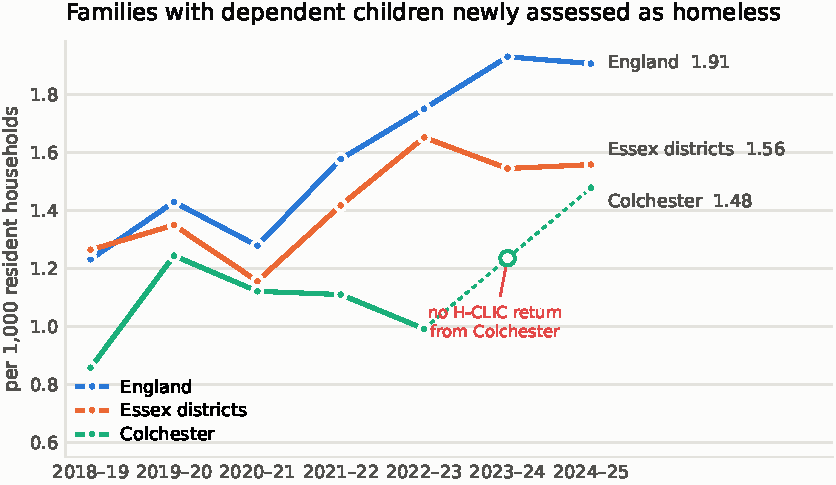
\includegraphics[width=0.70\textwidth]{../outputs/figures/fig_trend.pdf}
  \end{center}
  \vspace{-3mm}
  \begin{columns}[T,onlytextwidth]
    \begin{column}{0.55\textwidth}
      \scriptsize
      Across England the rate went from \lead{\EnglandRateFirst{} to
      \EnglandRateLast} per 1{,}000 households. In Colchester the number of
      families with children owed a relief duty rose from
      \ColchesterChildrenFirst{} to \ColchesterChildrenLast{}, an increase of
      \point{\ColchesterChildrenGrowth}.
    \end{column}
    \begin{column}{0.45\textwidth}
      \scriptsize
      \textcolor{critical}{\bfseries Colchester filed no H-CLIC return in
      2023--24,} one of \MissingReturnsPrev{} authorities that year. Sum the
      missing values to zero and the chart shows a collapse in family
      homelessness that never happened.
    \end{column}
  \end{columns}
\end{frame}

% =====================================================================
\begin{frame}{Finding 2: where prediction actually earns its place}
  \begin{center}
    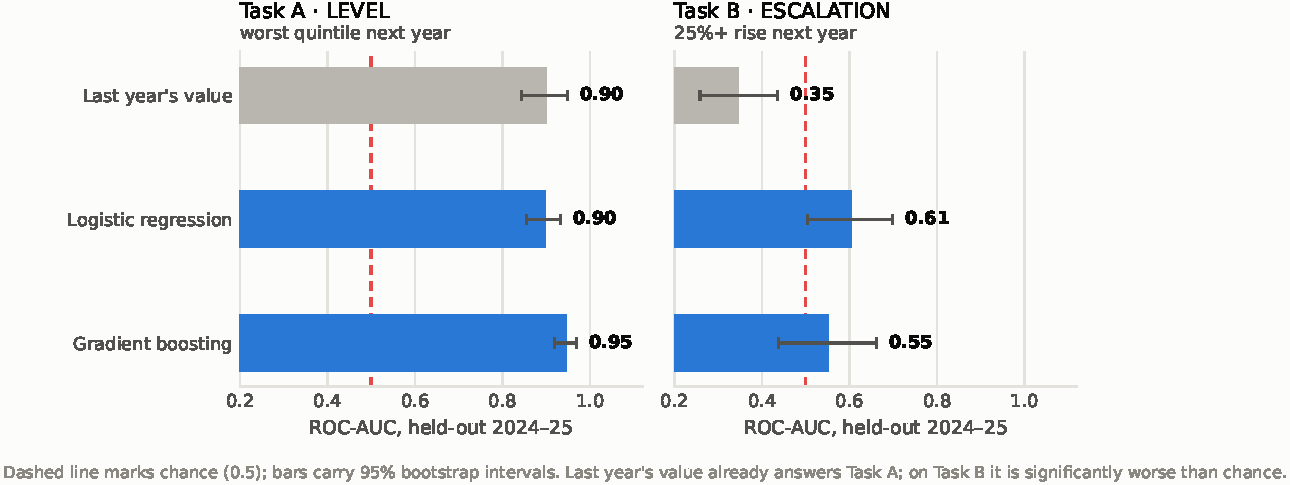
\includegraphics[width=0.78\textwidth]{../outputs/figures/fig_tasks.pdf}
  \end{center}
  \vspace{-1mm}
  \begin{columns}[T,onlytextwidth]
    \begin{column}{0.48\textwidth}
      \scriptsize
      \lead{Task A is a lookup.} Last year's value scores
      \LevelPersistenceAUC. A model reaches \LevelModelAUC, which is worth
      having for the calibration but not for the ranking. \textbf{There is no
      point building machine learning to answer a question that a sorted column
      already answers.}
    \end{column}
    \begin{column}{0.48\textwidth}
      \scriptsize
      \lead{Task B is the harder one.} The obvious heuristic, ``it went up
      last year so watch it'', scores \EscPersistenceAUC{}
      [\EscPersistenceLo--\EscPersistenceHi], \point{significantly worse than
      chance}. Rises tend to mean-revert, so acting on last year's increase
      sends help to the wrong places.
    \end{column}
  \end{columns}
\end{frame}

% =====================================================================
\begin{frame}{Finding 3: what that is worth to a team with a caseload}
  \begin{columns}[T,onlytextwidth]
    \begin{column}{0.56\textwidth}
      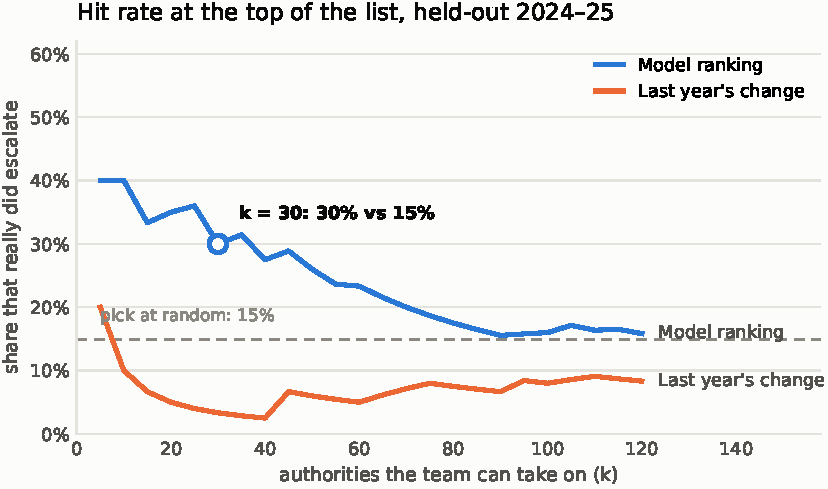
\includegraphics[width=\textwidth]{../outputs/figures/fig_precision_at_k.pdf}
    \end{column}
    \begin{column}{0.42\textwidth}
      \footnotesize
      A service cannot act on a ranking of the whole country. It works a list
      of fixed length, so the metric that matters is the \lead{hit rate at the
      top of that list} rather than AUC.
      \vspace{3mm}

      At $k=30$, \point{\EscModelPrecision{}} of the flagged areas really did
      escalate, against a base rate of \EscBaseRate. That is \lead{twice the
      yield} for the same effort.
      \vspace{3mm}

      The heuristic does worse than picking at random.
      \vspace{3mm}

      \smallcap{Held-out year \LastYear, $n=\EscTestN$. The absolute numbers
      are modest. I would rather show you an honest 2$\times$ than a polished
      0.9.}
    \end{column}
  \end{columns}
\end{frame}

% =====================================================================
\begin{frame}{Finding 4: the neighbourhood layer, and who a headline misses}
  \begin{columns}[T,onlytextwidth]
    \begin{column}{0.58\textwidth}
      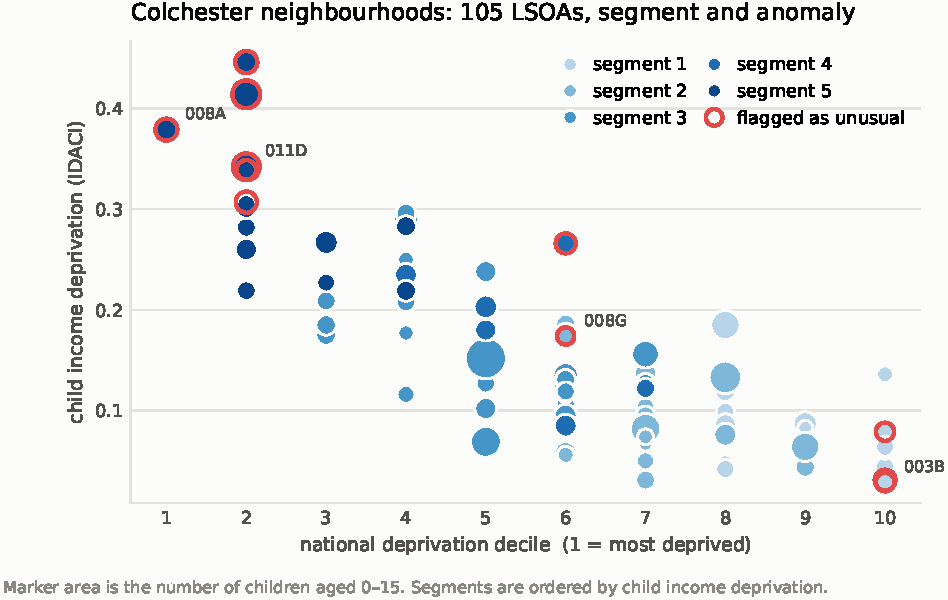
\includegraphics[width=\textwidth]{../outputs/figures/fig_colchester.pdf}
    \end{column}
    \begin{column}{0.40\textwidth}
      \footnotesize
      Colchester has \NumLSOA{} neighbourhoods and \NumChildren{} children
      aged 0--15. I grouped them into \NumSegments{} service profiles and used
      an Isolation Forest to flag \NumFlagged{} as unusual for Colchester.
      \vspace{3mm}

      \point{\NumHiddenFlagged{} of those \NumFlagged{} sit in the less
      deprived half of the country} and between them contain \HiddenChildren{}
      children. A triage that sorts on headline deprivation will not see them.
      \vspace{3mm}

      Risk and deprivation are correlated but they are not the same thing, and
      the gap between them is where earlier intervention becomes possible.
    \end{column}
  \end{columns}
\end{frame}

% =====================================================================
\begin{frame}{Built so that someone else can run it}
  \begin{columns}[T,onlytextwidth]
    \begin{column}{0.48\textwidth}
      \lead{Two layers}
      \begin{itemize}\footnotesize
        \item \NumModules{} library modules hold the logic: parsing, measure
              selection, boundary reconciliation, features, the models and
              their evaluation
        \item \NumStages{} stage scripts run them in order. Each reads one
              artefact, calls into the library, and writes the next
        \item Paths, years, split and thresholds are defined once, so the
              modelling stage and the dataset card cannot disagree about what
              the test year is
      \end{itemize}
    \end{column}
    \begin{column}{0.48\textwidth}
      \lead{Why it is worth the effort}
      \begin{itemize}\footnotesize
        \item \NumTests{} tests. The ones that matter most are on the label
              construction and the metrics, because that is where a bug
              changes a published number without changing anything visible
        \item Model configurations are read off the fitted pipelines, so the
              dashboard cannot describe a model nobody ran
        \item One command rebuilds the data, the models, the figures, this
              deck and the dashboard
      \end{itemize}
      \vspace{1mm}

      \smallcap{A research post leaves something behind. This is the shape I
      would want that to be in.}
    \end{column}
  \end{columns}
\end{frame}

% =====================================================================
\begin{frame}{What this rehearsal is not}
  \begin{columns}[T,onlytextwidth]
    \begin{column}{0.48\textwidth}
      \lead{Limits I would state in any report}
      \begin{itemize}\footnotesize
        \item The published statistics are aggregate, so this predicts areas
              rather than households. It is a test of method, not a finding
              about Colchester's families.
        \item Deprivation is fixed at 2019 while outcomes run to 2025.
        \item \MissingReturnsLast{} authorities did not report in \LastYear,
              and non-reporting is almost certainly not random.
        \item Effect sizes are modest and the intervals are wide.
      \end{itemize}
    \end{column}
    \begin{column}{0.48\textwidth}
      \lead{What changes with CBH's own data}
      \begin{itemize}\footnotesize
        \item Household level and monthly rather than annual, so the horizon
              becomes weeks. That is where prevention actually works
        \item Rent account trajectories, repairs, anti-social behaviour,
              contact history and tenancy events, all of which H-CLIC records
              only after the fact
        \item Free-text case notes, where transformer-based feature
              extraction genuinely earns its place
        \item Children's outcomes through ECC, such as school moves and
              attendance
      \end{itemize}
    \end{column}
  \end{columns}
\end{frame}

% =====================================================================
\begin{frame}{The first three months}
  \begin{columns}[T,onlytextwidth]

    % ---------------------------------------------------------------
    \begin{column}{0.305\textwidth}
      {\color{seriesone}\bfseries\large Month 1}\\[0.3mm]
      \smallcap{Access and understanding}\\[1.2mm]
      {\color{seriesone}\rule{\textwidth}{1.1pt}}\\[0.5mm]
      \footnotesize
      \begin{itemize}\setlength\itemsep{3pt}
        \item DPIA, sharing agreement, lawful basis
        \item Shadow officers; map how decisions get made
        \item Agree the outcome, and who acts on it
      \end{itemize}
    \end{column}

    % ---------------------------------------------------------------
    \begin{column}{0.305\textwidth}
      {\color{seriestwo}\bfseries\large Month 2}\\[0.3mm]
      \smallcap{The analysis asset}\\[1.2mm]
      {\color{seriestwo}\rule{\textwidth}{1.1pt}}\\[0.5mm]
      \footnotesize
      \begin{itemize}\setlength\itemsep{3pt}
        \item Link the data, with lineage and quality flags
        \item Map non-reporting and suppression
        \item Profile entries to temporary accommodation
      \end{itemize}
    \end{column}

    % ---------------------------------------------------------------
    \begin{column}{0.305\textwidth}
      {\color{seriesthree}\bfseries\large Month 3}\\[0.3mm]
      \smallcap{Baseline and pilot design}\\[1.2mm]
      {\color{seriesthree}\rule{\textwidth}{1.1pt}}\\[0.5mm]
      \footnotesize
      \begin{itemize}\setlength\itemsep{3pt}
        \item An interpretable baseline, validated prospectively
        \item Precision at real caseworker capacity
        \item Calibration and subgroup equity checks
      \end{itemize}
    \end{column}

  \end{columns}

  \vspace{2mm}
  {\color{inktwo!25}\rule{\textwidth}{0.6pt}}\\[1mm]
  {\color{inktwo}\scriptsize\textsc{what exists at the end}}\\[0.8mm]

  \begin{columns}[T,onlytextwidth]
    \begin{column}{0.305\textwidth}
      \scriptsize A governance route and an agreed outcome definition
    \end{column}
    \begin{column}{0.305\textwidth}
      \scriptsize A documented, reproducible dataset with a data dictionary
    \end{column}
    \begin{column}{0.305\textwidth}
      \scriptsize A practitioner-reviewed baseline and an evaluation design
    \end{column}
  \end{columns}
  \vspace{1mm}
\end{frame}

% =====================================================================
\begin{frame}{Four risks I would manage from day one}
  \begin{columns}[T,onlytextwidth]
    \begin{column}{0.48\textwidth}
      \begin{block}{Lead time}
        \footnotesize A correct prediction that arrives in the week a family
        presents as homeless is worth nothing. The evaluation has to score how
        early the warning came, not only whether it was right.
      \end{block}
      \begin{block}{Feedback loops}
        \footnotesize Once officers act on the score, the outcome data is
        contaminated, because a case that was successfully prevented looks
        exactly like a false positive. The evaluation design has to be agreed
        before the pilot starts.
      \end{block}
    \end{column}
    \begin{column}{0.48\textwidth}
      \begin{block}{Equity}
        \footnotesize A model trained on who was served will learn who tends
        to get served. Subgroup calibration needs to be a standing check rather
        than a one-off fairness audit.
      \end{block}
      \begin{block}{Proportionality}
        \footnotesize This is data about children. The test is not whether
        the model is accurate but whether a family ends up better off. That
        argues for a model an officer can interrogate, with a human decision at
        the end of it.
      \end{block}
    \end{column}
  \end{columns}
\end{frame}

% =====================================================================
\begin{frame}{What I would ask in week one}
  \begin{columns}[T,onlytextwidth]
    \begin{column}{0.48\textwidth}
      \lead{To Colchester Borough Homes}
      \begin{enumerate}\footnotesize
        \item What would the team do differently on a Monday morning if a
              household were flagged? If that is not yet settled, it is the
              first thing to design together.
        \item How many households can you realistically contact in a week?
              That number defines the metric.
        \item Which signals do experienced officers already trust? Those are
              the features worth starting from.
      \end{enumerate}
    \end{column}
    \begin{column}{0.48\textwidth}
      \lead{To the University and ECC}
      \begin{enumerate}\footnotesize
        \item What is the route to linking children's education and social
              care data, and how long does it take?
        \item What is already agreed on information governance, and what still
              has to be negotiated?
        \item Which publications and funding bids are we aiming at, so that
              the analysis can be designed for them from the start?
      \end{enumerate}
    \end{column}
  \end{columns}
  \vspace{4mm}
  \begin{center}
    \large\color{seriesone}\bfseries
    Thank you. I would be glad to take questions.
  \end{center}
\end{frame}

% =====================================================================
\appendix

\begin{frame}{Appendix: the pipeline}
  \scriptsize
  \begin{tabular}{@{}ll>{\raggedright\arraybackslash}p{0.50\textwidth}@{}}
    \toprule
    \textbf{Stage} & \textbf{Script} & \textbf{What it does} \\
    \midrule
    00 & \texttt{00\_download.py}      & Fetch H-CLIC and IoD2019 from gov.uk; checksum each file \\
    01 & \texttt{01\_extract\_hclic.py} & Parse seven publication spreadsheets with stacked merged headers, footnote markers and interleaved subtotals \\
    02 & \texttt{02\_build\_panel.py}   & Select measures by published header text, reconcile the 2019--2023 boundary changes and convert counts to rates \\
    03 & \texttt{03\_colchester\_lsoa.py} & Segment and anomaly-detect Colchester's neighbourhoods \\
    04 & \texttt{04\_model.py}          & Prospective backtest, both tasks, bootstrap intervals \\
    05 & \texttt{05\_figures.py}        & Every figure in this deck \\
    06 & \texttt{06\_facts.py}          & Every number in this deck, written out as \LaTeX{} macros \\
    07 & \texttt{07\_dashboard\_data.py} & The JSON behind the public dashboard \\
    08 & \texttt{08\_data\_profile.py}  & The dataset card, measured from the built artefacts \\
    \bottomrule
  \end{tabular}

  \smallcap{Most stages are under a hundred lines of wiring; the logic they
  call sits in the library. One command reproduces all of it, and no number
  here was typed by hand.}
\end{frame}

\begin{frame}{Appendix: the library the stages call}
  \scriptsize
  \begin{columns}[T,onlytextwidth]
    \begin{column}{0.48\textwidth}
      \begin{tabular}{@{}l>{\raggedright\arraybackslash}p{0.60\textwidth}@{}}
        \toprule
        \textbf{Module} & \textbf{What it owns} \\
        \midrule
        \texttt{config}    & Every path, year, split and threshold, defined once \\
        \texttt{sources}   & The gov.uk URLs, checked against the configured years \\
        \texttt{hclic}     & The publication-spreadsheet parser \\
        \texttt{panel}     & Measure selection, boundary maps, rate conversion \\
        \texttt{features}  & Design matrix and the two task labels \\
        \texttt{models}    & The model zoo, and what each member is for \\
        \bottomrule
      \end{tabular}
    \end{column}
    \begin{column}{0.48\textwidth}
      \begin{tabular}{@{}l>{\raggedright\arraybackslash}p{0.58\textwidth}@{}}
        \toprule
        \textbf{Module} & \textbf{What it owns} \\
        \midrule
        \texttt{mlp}            & The Monte-Carlo dropout network \\
        \texttt{evaluation}     & The backtest, the metrics, the bootstrap \\
        \texttt{neighbourhoods} & Segmentation and anomaly detection \\
        \texttt{plotting}       & Design tokens and figure plumbing \\
        \texttt{profiling}      & The dataset card, measured from the artefacts \\
        \texttt{export}         & JSON for the dashboard, macros for these slides \\
        \bottomrule
      \end{tabular}
    \end{column}
  \end{columns}
  \vspace{3mm}

  \smallcap{Installed as a package, so the stages, the tests and a notebook
  all import the same code. Splitting it this way is what makes the parts
  where a bug would be invisible directly testable.}
\end{frame}

\begin{frame}{Appendix: what the tests actually check}
  \begin{columns}[T,onlytextwidth]
    \begin{column}{0.48\textwidth}
      \footnotesize
      \lead{Where a silent bug would hurt most}
      \begin{itemize}
        \item A label taken from the wrong year, or from a neighbouring
              authority after a grouped shift
        \item A quantile cutoff recomputed on the year being scored, which
              would fix its prevalence at the nominal quintile by construction
        \item A relative rise computed from a zero baseline
        \item A missing return arriving as a zero
      \end{itemize}
      \vspace{1mm}

      \smallcap{Each of those has a test whose answer can be worked out by
      hand.}
    \end{column}
    \begin{column}{0.48\textwidth}
      \footnotesize
      \lead{And the fragile inputs}
      \begin{itemize}
        \item The spreadsheet parser, against a synthetic sheet carrying every
              awkward feature of the real ones: a banner title, stacked merged
              headers, a percentage sharing a header with its count, region
              subtotals above the authorities
        \item Measure selection: the shortest matching header wins, a measure
              stays inside its own table, an unresolved measure becomes null
              rather than zero
        \item The boundary maps: no district claimed by two successors, and
              none both created and retired
      \end{itemize}
    \end{column}
  \end{columns}
\end{frame}

\begin{frame}{Appendix: boundary and coverage reconciliation}
  \begin{columns}[T,onlytextwidth]
    \begin{column}{0.48\textwidth}
      \footnotesize
      \lead{Local authorities move.} There were 326 districts in \FirstYear{}
      and 296 in \LastYear, while IoD2019 is published on 2019 boundaries.
      \begin{itemize}
        \item Seven successor authorities (Buckinghamshire, the two
              Northamptonshires, the two Cumbrias, North Yorkshire and
              Somerset) rebuilt by population-weighting their predecessors'
              LSOAs
        \item Fourteen districts abolished in April 2019 mapped onto their
              successors
        \item Every authority-year then carries a deprivation score
      \end{itemize}
    \end{column}
    \begin{column}{0.48\textwidth}
      \footnotesize
      \lead{Measures move too.} 251 of the 252 measure-years resolve by
      matching published header text rather than column position, so a layout
      change raises an error instead of quietly shifting a feature.
      \vspace{2mm}

      The one gap is real: Section 21 notices were not collected in
      \FirstYear.
      \vspace{2mm}

      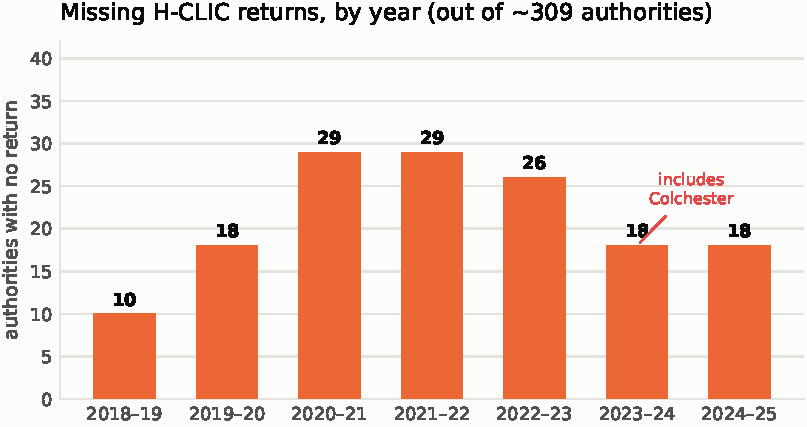
\includegraphics[width=\textwidth]{../outputs/figures/fig_data_quality.pdf}
    \end{column}
  \end{columns}
\end{frame}

\begin{frame}{Appendix: the models that predict}
  \scriptsize
  \begin{tabular}{@{}>{\raggedright\arraybackslash}p{0.24\textwidth}
                    >{\raggedright\arraybackslash}p{0.32\textwidth}
                    >{\raggedright\arraybackslash}p{0.37\textwidth}@{}}
    \toprule
    \textbf{Model} & \textbf{Configuration} & \textbf{Why it is there} \\
    \midrule
    \lead{Logistic regression}
      & Median impute, standardise, L2 at $C=0.3$
      & The interpretable reference and the source of the driver chart.
        Strongest of the four on escalation \\
    \addlinespace
    \lead{Gradient boosting}
      & Histogram-based, depth 3, 300 iterations, $\eta=0.06$
      & Handles the 14\% missingness natively rather than imputing values that
        were never collected \\
    \addlinespace
    \lead{\quad + calibration}
      & Isotonic, 3-fold
      & A triage score is read as a probability, so it has to be one.
        Brier \BrierBefore{} to \BrierAfter \\
    \addlinespace
    \lead{Neural network}
      & PyTorch MLP, 64--32, dropout 0.3, reweighted loss, early stopping,
        Monte-Carlo dropout at inference
      & Competitive without winning: 0.93 and 0.59, both inside the best
        model's interval. It is here for the uncertainty, since each authority
        gets a spread rather than only a score \\
    \bottomrule
  \end{tabular}
  \vspace{1mm}

  \smallcap{Each is fitted twice, once per task. No stacking: the differences
  sit inside their confidence intervals.}
\end{frame}

% =====================================================================
\begin{frame}{Appendix: the baselines, and the neighbourhood models}
  \scriptsize
  \begin{tabular}{@{}>{\raggedright\arraybackslash}p{0.24\textwidth}
                    >{\raggedright\arraybackslash}p{0.30\textwidth}
                    >{\raggedright\arraybackslash}p{0.39\textwidth}@{}}
    \toprule
    \textbf{Model} & \textbf{Configuration} & \textbf{Why it is there} \\
    \midrule
    \lead{Persistence}
      & Last year's value, or last year's change
      & What a service already has without any analytics. It answers Task A,
        and on Task B it is significantly worse than chance. Two of my three
        findings come from this row \\
    \addlinespace
    \lead{Prevalence}
      & Predict the base rate for everyone
      & Fixes the floor, so that ``\EscModelPrecision{} of the flagged areas''
        has something to be compared against \\
    \midrule
    \lead{$k$-means}
      & Nine standardised deprivation domains, $k=5$ by silhouette,
        restricted to $k \geq 4$
      & Neighbourhood service profiles. $k=2$ scores higher but only recovers
        deprived and not deprived, which the service already knows \\
    \addlinespace
    \lead{Isolation Forest}
      & 500 trees, 10\% contamination, same nine features
      & Finds neighbourhoods unusual \emph{for Colchester}. Contamination is
        fixed rather than tuned: with 105 points and no ground truth there is
        nothing honest to tune against \\
    \bottomrule
  \end{tabular}
\end{frame}

% =====================================================================
\begin{frame}{Appendix: what the model keys on}
  \begin{columns}[T,onlytextwidth]
    \begin{column}{0.62\textwidth}
      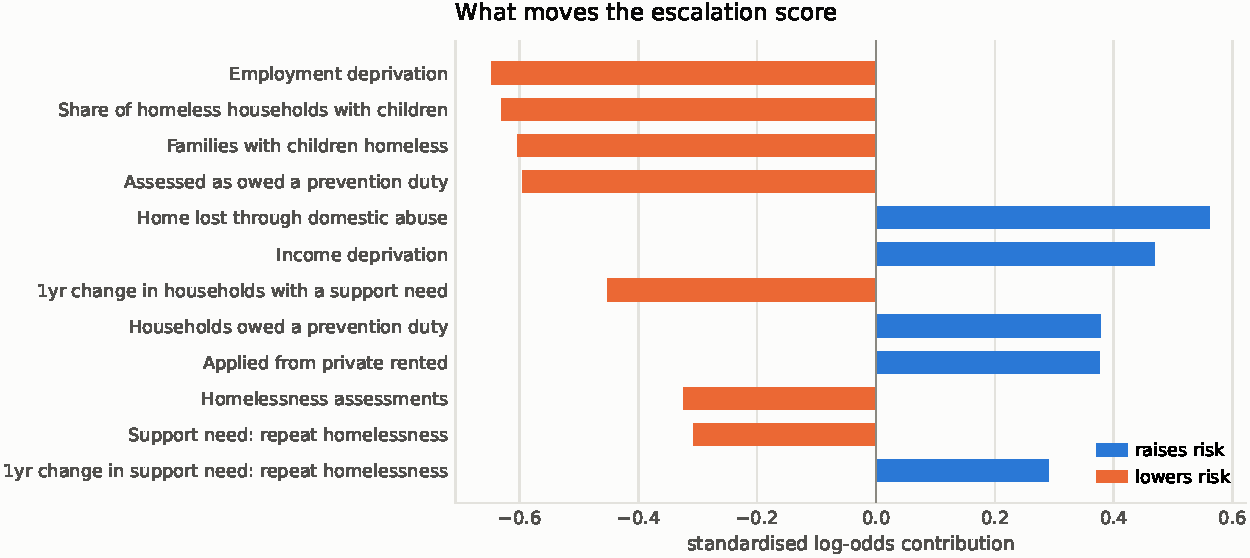
\includegraphics[width=\textwidth]{../outputs/figures/fig_drivers.pdf}
    \end{column}
    \begin{column}{0.36\textwidth}
      \footnotesize
      Domestic abuse as a route out of the last settled home \lead{raises}
      escalation risk. Areas that are already high on family homelessness
      \lead{lower} it, which is the same mean reversion that makes the
      persistence heuristic anti-predictive.
      \vspace{3mm}

      The directions are stable and readable, which is what an officer needs in
      order to disagree with the model.
    \end{column}
  \end{columns}
\end{frame}

\begin{frame}{Appendix: does the score mean what it says?}
  \begin{columns}[T,onlytextwidth]
    \begin{column}{0.45\textwidth}
      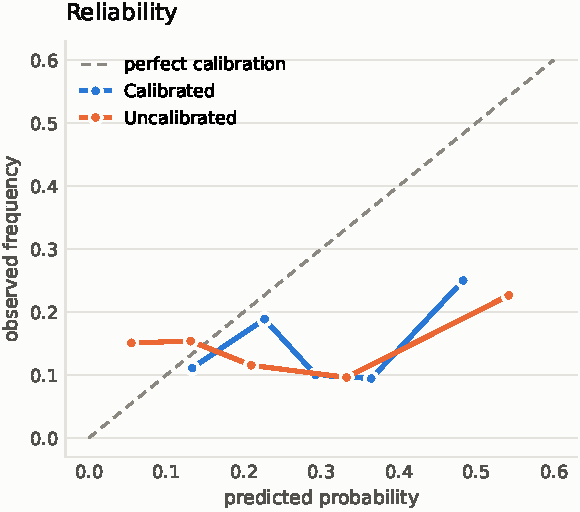
\includegraphics[width=\textwidth]{../outputs/figures/fig_calibration.pdf}
    \end{column}
    \begin{column}{0.53\textwidth}
      \footnotesize
      Whoever acts on a triage score will read it as a probability, so it had
      better be one. Isotonic calibration takes the Brier score from
      \BrierBefore{} to \BrierAfter{} on the level task.
      \vspace{3mm}

      A score that ranks well but is badly calibrated misleads a service about
      how many families are actually at risk, and therefore about how much
      capacity to commit. \lead{That is the part I would not compromise on.}
      \vspace{3mm}

      Selective prediction follows the same reasoning. A model that abstains
      where it is uncertain is more useful than one that always answers.
    \end{column}
  \end{columns}
\end{frame}

\begin{frame}{Appendix: sources}
  \footnotesize
  \begin{itemize}
    \item MHCLG, \emph{Statutory homelessness: detailed local authority-level
          tables}, financial years \FirstYear{} to \LastYear.
          \smallcap{gov.uk/government/statistical-data-sets/live-tables-on-homelessness}
    \item MHCLG, \emph{English Indices of Deprivation 2019}. File 7 (LSOA
          scores, ranks, deciles and population denominators) and File 10
          (lower-tier local authority summaries).
          \smallcap{gov.uk/government/statistics/english-indices-of-deprivation-2019}
    \item ONS, register of local government reorganisations 2020--2023, for
          the boundary crosswalk.
  \end{itemize}
  \vspace{3mm}
  All released under the Open Government Licence v3.0. No personal or
  household-level data was used, accessed or held at any point in this
  exercise.
\end{frame}

\end{document}
